% Chapter Template

\chapter{Introduction} % Main chapter title

\label{Chapter2} % Change X to a consecutive number; for referencing this chapter elsewhere, use \ref{ChapterX}

\lhead{Chapter 1. \emph{Introduction}} % Change X to a consecutive number; this is for the header on each page - perhaps a shortened title

%----------------------------------------------------------------------------------------
%	SECTION 1
%----------------------------------------------------------------------------------------

\section{Motivation}

Scramjet engines are on the forefront of supersonic transportation development because of their simplicity and promising outlook for steady and reliable supersonic combustion. These engines differ from typical subsonic jet engines, as scramjets have no moving parts and simply rely on shock waves produced at these supersonic speeds to compress the intake air and provide the means for ignition. Shown in Figure \ref{fig:scramjet} is a diagram of a typical scramjet engine.

One challenge facing the production of these engines is producing steady combustion. Much like keeping a match lit in a hurricane, keeping a flame stabilized at supersonic speeds is quite difficult. One proposed method of flame stabilization is a rectangular cavity. These cavities, are able provide a re-circulation zone with high temperatures and combustion radicals for strong combustion to occur. Many experimental studies have tested the flame-holding abilities of cavities in strong combustion cases \cite{ben2000experimental,ben2001cavity,do2009plasma,yilmaz2013investigation}. Strong combustion occurs when the fuel-air mixture is optimized for efficient fuel burning. The mixture in strong combustion cases occur in proper stoichiometric proportions. These studies focused on cavity dimensions and how the length to depth ratio, L/D, affects key ignition and flame holding characteristics, such as stagnation pressure, stagnation temperature, fuel air mixture, and residence time. Ben-Yakar concluded that with L/D ratios between 4 and 10, strong combustion can be sustained in these cavities for total enthalpy flight conditions of Mach 8, 10, and 13\cite{ben2001cavity}. Also noted in several investigations is the presence of strong acoustic waves\cite{unalmis2004cavity,heller1996letter,williams2007supersonic, mcgregor1970drag,luo2011drag, sato1999advanced}. 

Similar to blowing air over an empty bottle to create a tone, the freestream air traveling over and interacting with these cavities produces acoustic waves. In these cavities, a shear layer develops between the high speed freestream and the slower, re-circulating air in the cavity. As the shear layer travels downstream, it begins to drop. By the time the shear layer reaches the downstream wall of the cavity, it has lowered to a point where the interaction of the shear layer with the downstream wall of the cavity produces strong pressure waves, which propagate upstream, ultimately resonating within the cavity. 

Other experimental studies have investigated the acoustic properties of these cavities \cite{unalmis2004cavity,heller1996letter,williams2007supersonic, mcgregor1970drag,luo2011drag}. These investigations concluded that the acoustic waves generated by supersonic cavities produce several undesirable effects. One effect, investigated by McGregor is the induced drag associated with rectangular cavities. The effect of pressure waves within these cavities can increase the drag by as much as 250\% \cite{mcgregor1970drag}. These acoustic waves can also have an adverse effect on equipment and the crew. At low frequencies, the resonating acoustic waves can cause structural damage to the engine. At high frequencies, these waves can cause uneasiness in crew members \cite{mcgregor1970drag}.

Conclusions drawn from these investigations have led to the desire to suppress these acoustic waves. Suppressing these waves would reduce drag on the engine and cause less damage to the engine or the crew. However, these acoustic waves could have the potential to assist in combustion when conditions for weak combustion are present. Weak combustion, as is studied in this investigation, is at lean fuel air mixture conditions. Sato et al.\cite{sato1999advanced} investigated the enhancement of mixing due to acoustic waves. They concluded that mixing was enhanced by these acoustic waves and the rate of enhancement was controlled by the cavity's shape. However, the investigations performed by Sato et al. did not include the cavity as a flame-holder. The cavity was only used to produce the mixing enhancing acoustic waves. 

One study, though, focused on the ability of cavity-induced acoustic waves to enhance mixing \cite{sato1990advanced}. Their experimental setup, as shown in Figure \ref{fig:sato} shows that the wall-mounted cavities were used exclusively as acoustic wave generators to enhance the mixing of the freestream and the injected gas. Their study showed that the cavity acoustic waves produced had enough energy to enhance mixing. This study will attempt to combine the flame-holding characteristics of these cavities with the acoustic wave assisted mixing. The acoustic waves generated inside the cavity should have nearly the same strength as the waves that escaped the cavity in Sato's study. 

Few, if any, experimental studies have investigated the acoustic properties of these cavities as they assist in mixing and the enhancement of combustion at lean conditions. This investigation is broken into three parts, which together will provide a clear interpretation of a cavity's suitability as an effective flame holder during weak combustion conditions. 


%-----------------------------------
%	SUBSECTION 1
%-----------------------------------
\subsection{Phase 1}

The first part of the investigation isolated the acoustic properties of the cavities. The frequency of a cavity can be estimated using an empirical equation derived by Heller and Delfs \cite{heller1996letter}, as shown in Equation \ref{eq:freq}. This equation is estimated to be able to predict the frequency within the cavity $\pm$10\%\cite{heller1996letter}.

\begin{equation}
f_m = \frac{m-\alpha}{\{M_{\infty}/\sqrt{1+[(\gamma_{\infty}-1)/2]M_{\infty}^2}+1/k\}} \cdot \frac{U_\infty}{L}
\label{eq:freq}
\end{equation}

Depending on the mode of the strongest acoustic waves, frequencies of these waves were expected to be between \textbf{FREQUENCY RANGE}. For this phase, three L/D ratios were investigated: 5, 7, and 9. From the equation, it can be seen that the frequency generated by the cavity is a function of the freestream test gas conditions and length of the cavity. Keeping the freestream conditions nearly identical while changing the length of the cavity produced different frequencies within the cavity. Data from these tests led to the direct comparison of the acoustic properties of the cavities, such as frequency and relative strength, as a function of cavity frequency. Also investigated at each of the L/D ratios was an angled downstream wall to observe the passive suppression of the normally present acoustic waves.

%-----------------------------------
%	SUBSECTION 2
%-----------------------------------

\subsection{Phase 2}

The second part of the investigation was used to isolate the combustion and flame-holding properties of the cavities.


%-----------------------------------
%	SUBSECTION 3
%-----------------------------------

\subsection{Phase 3}

The third part of the investigation has yet to be tested. This phase is used to observe the effect that the acoustic waves have on the flame-holding characteristics of the cavities in a non-stoichiometric fuel-air mixture. For these experiments, both flat and angled wall cavities will be tested at the same conditions. Shown by results of Phase 1, the angled walls do suppress the propagating acoustic waves within the cavity, so any observable differences between the results of the angled versus flat downstream wall will be assumed to be due to the cavity acoustics. Ideally, the results of these tests would be to show that the flat downstream wall, and thus the cavity acoustics, do enhance the mixing of the fuel and air, producing stronger combustion than the angled downstream wall. More details about Phase 3 are included in the Future Works section of this thesis, Chapter \ref{Chapter6}.


%-------------------------------------------------------
%    FIGURES
%------------------------------------------------------
\newpage

\begin{figure}
\centering
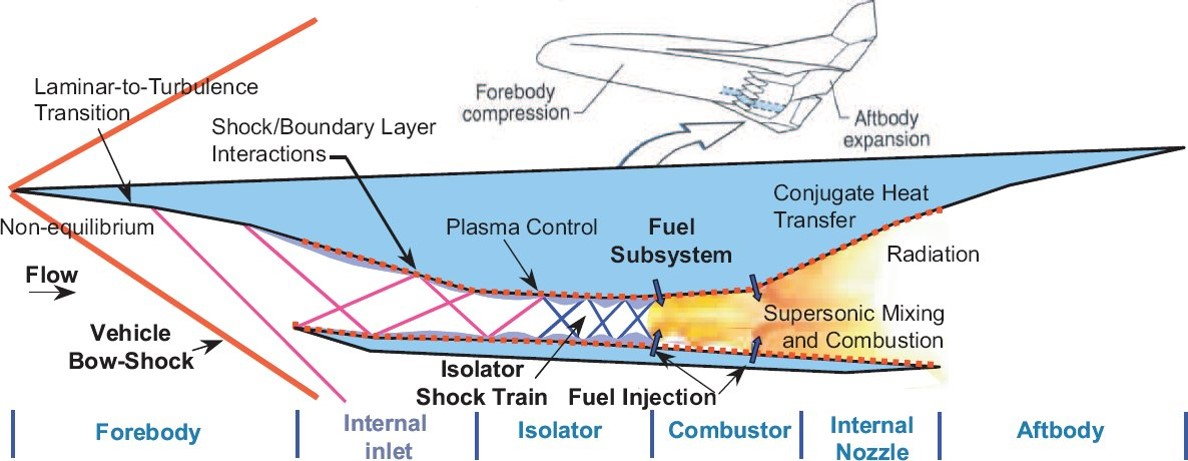
\includegraphics[width=\textwidth]{Figures/scramjet.jpg}
\caption[Scramjet Diagram]{Diagram of a typical scramjet engine, showing shocks produced within the engine. \cite{scramjetFig}}
\label{fig:scramjet}
\end{figure}


\begin{figure}
\centering
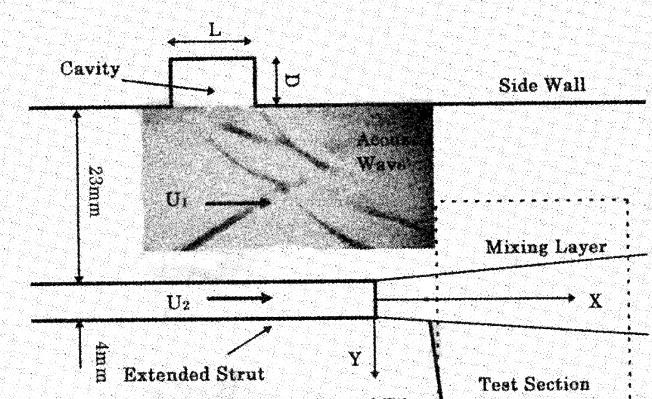
\includegraphics[height=3in]{Figures/CavMix.jpg}
\caption[Cavity-Actuated Mixing]{Mixing enhanced by acoustic waves produced by a side wall-mounted cavity \cite{sato1999advanced}}
\label{fig:sato}
\end{figure}

